\begin{minipage}{0.75\linewidth}
\begin{figure}[h]
    \centering
    \begin{adjustbox}{max width=1.0\linewidth, keepaspectratio}
        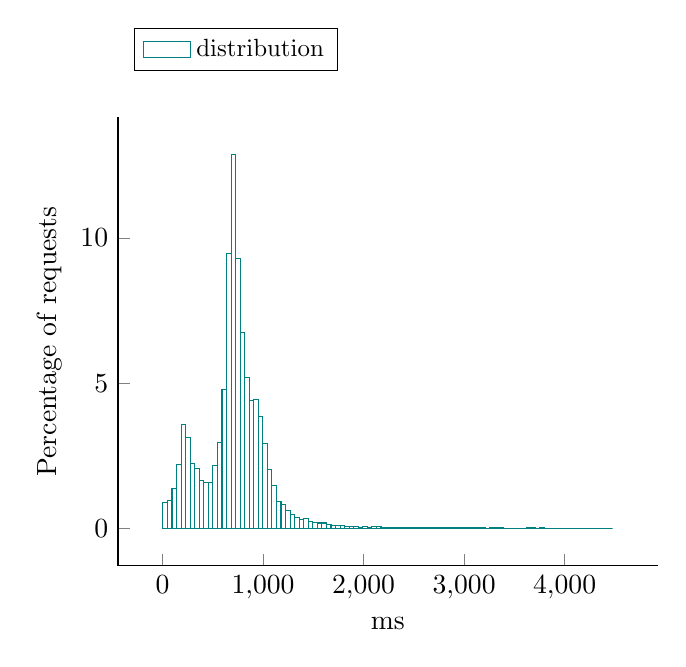
\begin{tikzpicture}
            \begin{axis}[ylabel = Percentage of requests, 
xlabel = ms, 
legend style = {nodes={scale=0.9, transform shape}, at={(0.03,1.2)}, anchor=north west, draw=black, fill=white, align=left, legend columns=3},
area style, mark size = 0pt,
 cycle list name = exotic,
  axis lines* = left]
		\addplot +[ybar interval] coordinates {
			 (4, 0.901296)
			 (49.19, 0.96858)
			 (94.38, 1.3582)
			 (139.57, 2.19221)
			 (184.76, 3.5645)
			 (229.95, 3.11698)
			 (275.14, 2.21881)
			 (320.33, 2.07486)
			 (365.52, 1.64455)
			 (410.71, 1.56475)
			 (455.9, 1.57414)
			 (501.09, 2.16718)
			 (546.28, 2.95112)
			 (591.47, 4.76936)
			 (636.66, 9.46517)
			 (681.85, 12.8685)
			 (727.04, 9.29305)
			 (772.23, 6.74563)
			 (817.42, 5.18089)
			 (862.61, 4.40008)
			 (907.8, 4.4345)
			 (952.99, 3.83677)
			 (998.18, 2.92295)
			 (1043.37, 2.0373)
			 (1088.56, 1.46773)
			 (1133.75, 0.912249)
			 (1178.94, 0.81054)
			 (1224.13, 0.621205)
			 (1269.32, 0.483508)
			 (1314.51, 0.384928)
			 (1359.7, 0.311385)
			 (1404.89, 0.347374)
			 (1450.08, 0.231583)
			 (1495.27, 0.208112)
			 (1540.46, 0.181511)
			 (1585.65, 0.183076)
			 (1630.84, 0.129874)
			 (1676.03, 0.109532)
			 (1721.22, 0.111097)
			 (1766.41, 0.0923202)
			 (1811.6, 0.0578957)
			 (1856.79, 0.0704137)
			 (1901.98, 0.0610252)
			 (1947.17, 0.0406835)
			 (1992.36, 0.0547662)
			 (2037.55, 0.0391187)
			 (2082.74, 0.056331)
			 (2127.93, 0.0594605)
			 (2173.12, 0.0391187)
			 (2218.31, 0.031295)
			 (2263.5, 0.0422482)
			 (2308.69, 0.0344245)
			 (2353.88, 0.037554)
			 (2399.07, 0.0359892)
			 (2444.26, 0.0328597)
			 (2489.45, 0.0297302)
			 (2534.64, 0.0266007)
			 (2579.83, 0.0156475)
			 (2625.02, 0.031295)
			 (2670.21, 0.0219065)
			 (2715.4, 0.025036)
			 (2760.59, 0.0203417)
			 (2805.78, 0.0172122)
			 (2850.97, 0.012518)
			 (2896.16, 0.018777)
			 (2941.35, 0.0297302)
			 (2986.54, 0.0140827)
			 (3031.73, 0.012518)
			 (3076.92, 0.0140827)
			 (3122.11, 0.0172122)
			 (3167.3, 0.012518)
			 (3212.49, 0.006259)
			 (3257.68, 0.0109532)
			 (3302.87, 0.0093885)
			 (3348.06, 0.012518)
			 (3393.25, 0.006259)
			 (3438.44, 0.006259)
			 (3483.63, 0.00469425)
			 (3528.82, 0.00156475)
			 (3574.01, 0)
			 (3619.2, 0.0093885)
			 (3664.39, 0.0109532)
			 (3709.58, 0.006259)
			 (3754.77, 0.0093885)
			 (3799.96, 0.006259)
			 (3845.15, 0.00782375)
			 (3890.34, 0.00782375)
			 (3935.53, 0.00156475)
			 (3980.72, 0.00782375)
			 (4025.91, 0.0031295)
			 (4071.1, 0.0031295)
			 (4116.29, 0.00156475)
			 (4161.48, 0.0031295)
			 (4206.67, 0.0031295)
			 (4251.86, 0.00469425)
			 (4297.05, 0.00156475)
			 (4342.24, 0.00156475)
			 (4387.43, 0.00156475)
			 (4432.62, 0)
			 (4477.81, 0)
		};
\addlegendentry{distribution};
           \end{axis}
      \end{tikzpicture}
  \end{adjustbox}
  \caption{Response time distribution - req = ALL}
\end{figure}
\end{minipage}\hfill\begin{minipage}{0.18\linewidth}
\begin{table}[h]
\begin{tabular}{|cc|}
\hline
\textbf{} & \textbf{ms}\\ \hline
 \Xhline{0.005\arrayrulewidth}
min & 4\\
 \Xhline{0.005\arrayrulewidth}
max & 4523\\
 \Xhline{0.005\arrayrulewidth}
mean & 716\\
 \Xhline{0.005\arrayrulewidth}
std & 355\\
\hline
\hline
 \Xhline{0.005\arrayrulewidth}
25th & 573\\
 \Xhline{0.005\arrayrulewidth}
50th & 715\\
 \Xhline{0.005\arrayrulewidth}
75th & 866\\
 \Xhline{0.005\arrayrulewidth}
80th & 918\\
 \Xhline{0.005\arrayrulewidth}
85th & 970\\
 \Xhline{0.005\arrayrulewidth}
90th & 1039\\
 \Xhline{0.005\arrayrulewidth}
95th & 1198\\
 \Xhline{0.005\arrayrulewidth}
99th & 1924\\
\hline
\end{tabular}
\caption{Response time}
\end{table}
\end{minipage}\hfill